% Source: Gerzensee "Dynamic Programming" slides 2-63 (the range of dynamic
% economic problems; the sequential problem and its constraints; the value
% function; stationarity and the prime notation; the policy function; Bellman's
% principle quoted from Bellman (1957, p. 83); the Bellman equation and the
% operator T; the contraction argument via Blackwell's monotonicity and
% discounting conditions verified line by line; value function iteration with the
% geometric error bound; the first-order condition and the envelope formula with
% the full derivation; the cake-eating problem in its two state/control
% formulations, its grid implementation and its closed-form log solution; the
% Ramsey growth model, its Euler equation and steady state; the Lucas asset
% pricing model, the consumer's problem, the equilibrium constraints, the
% consumption-based pricing equation, the stochastic discount factor, Lucas'
% indirect approach, the contraction proof for T, and the log-utility closed form).
% Supplementary: Fukuda (2026), Ch. 15 (pp. 513-...; Sec. 15.1.1-15.1.4, 15.2).
% Code: Supplementary/codes/DP_cake_eating.m, DP_cake_eating_CRRA.m,
% DP_cake_eating_plot_iterations.m, deterministic_Ramsey_growth.m,
% Lucas_Tree_DP.m, Lucas_Tree_DP_Octave.m.
% External references actually cited in this chapter: Bellman (1957),
% Benveniste-Scheinkman (1979), Rockafellar (1970), Stokey et al. (1989).

\chapter{Discrete-Time Dynamic Programming}
\label{ch:dynamic}

\section{The Sequential Problem}\label{sec:dyn-sequential}

\begin{definition}[Sequential problem]\label{def:sequential-problem}
	Let $r\colon\R^{n}\times\R^{k}\to\R$ be the \dfnas{return
		function}{return function}, $g\colon\R^{n}\times\R^{k}\to\R^{n}$ the \dfnas{transition function}{transition
		function} and $\beta\in(0,1)$ the \dfnas{discount factor}{discount
		factor}. The \dfnas{sequential problem}{sequential problem}
	from an initial state $x_0\in\R^{n}$ is
	\begin{equation}\label{eq:sequential-problem}
		\sup_{(u_t)_{t=0}^{\infty}}\ \sum_{t=0}^{\infty}\beta^{t}r(x_t,u_t)
		\qquad\st\quad
		x_{t+1}=g(x_t,u_t)\ \text{ for every }t\geq0,\quad x_0\ \text{given}.
	\end{equation}
	Its value is the \dfnas{value function}{value function}
	$V(x_0)$. The variable $x_t\in\R^{n}$ is the \dfn{state}, $u_t\in\R^{k}$ the
	\dfn{control}, and a \dfnas{policy function}{policy function} is a map
	$h\colon\R^{n}\to\R^{k}$ prescribing $u=h(x)$.
	\nidx{valuefunction}{$V$, value function}
	\nidx{policyfunction}{$h$, policy function}
\end{definition}

\begin{assumption}[Standing hypotheses]\label{ass:dyn}
	Throughout this chapter:
	\begin{enumerate}[(i)]
		\item the state lies in a set $X\subseteq\R^{n}$ and the feasible controls at
		      $x$ form a set $\Gamma(x)\subseteq\R^{k}$, defining a correspondence
		      $\Gamma\colon X\rightrightarrows\R^{k}$ that is non-empty- and
		      compact-valued and continuous;
		\item the transition $g\colon\gph\Gamma\to\R^{n}$ is continuous and satisfies
		      $g(x,u)\in X$ for every $x\in X$ and $u\in\Gamma(x)$, so the problem is
		      well defined;
		\item $r$ is continuous and bounded on $\gph\Gamma$;
		\item $\beta\in(0,1)$.
	\end{enumerate}
\end{assumption}

Continuity of $g$ in (ii) enters at one point, and that point carries the
chapter: the Bellman operator
\eqref{eq:bellman-max} sends $v$ to a supremum of
$r(x,u)+\beta v(g(x,u))$, and the composite $(x,u)\mapsto v(g(x,u))$ is
continuous on $\gph\Gamma$ only if $g$ is. Without it $T$ need not map bounded
continuous functions to bounded continuous functions,
\autoref{thm:berge-maximum} cannot be applied to the maximisation, and neither
the continuity of $V$ nor the upper hemicontinuity of the policy correspondence
in \autoref{prop:bellman-well-defined} is available. The contraction argument itself would
survive on the space of bounded measurable functions, but the identification of
$V$ as a continuous function would not.

Boundedness in (iii) is what makes the infinite sum in
\eqref{eq:sequential-problem} converge absolutely: $\abs{r}\leq\bar r$ gives
$\bigl|\sum_t\beta^{t}r(x_t,u_t)\bigr|\leq\bar r/(1-\beta)$ for every feasible
sequence, so the supremum is finite and no ordering or summability question
arises. It is a genuine restriction --- it excludes $\log$ utility on an
unbounded state space, and the cake-eating problem of
\autoref{sec:dyn-cake} violates it as $w\downarrow0$ --- and
\autoref{rem:unbounded-returns} records what survives without it.

\begin{remark}[Stationarity and the prime notation]\label{rem:stationarity}
	The problem is \dfnas{stationary problem}{stationary}: neither $r$, $g$ nor
	$\Gamma$ depends on $t$, and the horizon is infinite at every date. Therefore
	\[
		V(x_t)=\beta^{-t}\sup_{(u_\tau)_{\tau\geq t}}\
		\sum_{\tau=t}^{\infty}\beta^{\tau}r(x_\tau,u_\tau)
	\]
	subject to the same constraints: the problem faced at date $t$ in state $x_t$ is
	the same problem faced at date $0$ in state $x_0=x_t$. Only the state matters,
	not the date at which it is reached, and one may therefore drop time subscripts
	and write $x$ for today's state and $x'$ for tomorrow's
	\autocite[slide 8]{fukuda2026dynamic}. Every statement about $V$ and $h$ below
	is a statement about functions of the state alone; the reduction from a sequence
	problem in infinitely many variables to a functional equation in one is the
	entire content of the method.
\end{remark}

\section{Bellman's Principle of Optimality}\label{sec:dyn-bellman}

\begin{quote}
	``An optimal policy has the property that whatever the initial state and initial
	decision are, the remaining decisions must constitute an optimal policy with
	regard to the state resulting from the first decision.''
	\autocite[p.~83]{bellman1957dynamic}
\end{quote}

\begin{definition}[Bellman operator]\label{def:bellman-operator}
	Under \autoref{ass:dyn}, write
	$\Cbspace{X}\eqdef\Cspace{X}{\R}\cap\Bspace{X}{\R}$ for the space of bounded
	continuous functions $X\to\R$ with the supremum norm, and define $T$ on it by
	\nidx{Cb}{$\Cbspace{X}$, bounded continuous functions on $X$}
	\begin{equation}\label{eq:bellman-max}
		(TW)(x)\eqdef\max_{u\in\Gamma(x)}\ \bigl\{r(x,u)+\beta W\bigl(g(x,u)\bigr)\bigr\},
		\qquad x\in X .
	\end{equation}
	A function $W$ with $W=TW$ solves the \dfnas{Bellman equation}{Bellman equation}.
	\nidx{bellmanoperator}{$T$, Bellman operator}
\end{definition}

Definition \eqref{eq:bellman-max} is \eqref{eq:bellman-operator} of
\autoref{ch:completeness} with the supremum replaced by a maximum. The
replacement is a theorem, not a convention: \autoref{ass:dyn} makes the
constraint correspondence compact-valued and the objective continuous, so
\autoref{prop:bellman-well-defined} shows the supremum is attained. Where it is
not, every statement below about the policy correspondence fails while the
contraction argument of \autoref{prop:bellman-contraction} survives unchanged.

\begin{remark}[Which space $T$ acts on]\label{rem:dyn-function-space}
	Three spaces of functions on $X$ appear in dynamic programming and they are
	not interchangeable. The largest is $\Bspace{X}{\R}$, the bounded functions,
	complete in the supremum norm by \autoref{thm:B-complete}; the smallest is
	$\Cbspace{X}$, the bounded continuous ones, a closed subspace and hence
	complete by \autoref{prop:C-complete}; between them sits the space of bounded
	\emph{measurable} functions, also closed under uniform limits. The Bellman
	operator is a contraction of modulus $\beta$ on any of the three by the same
	two-line Blackwell argument, since neither monotonicity nor discounting sees
	the regularity of $W$. What differs is the object the fixed point turns out
	to be. On $\Bspace{X}{\R}$ the fixed point is bounded and nothing more, and
	no policy need be selectable from $H_V$. On $\Cbspace{X}$ one needs $T$ to
	preserve continuity, which is where \autoref{ass:dyn} and Berge's theorem are
	spent, and the reward is that $V$ is continuous and $H_V$ is upper
	hemicontinuous with compact values. On the bounded measurable functions $T$
	preserves measurability under weaker hypotheses on $\Gamma$, and selecting a
	policy from $H_V$ then requires a measurable selection theorem rather than
	Berge's; this is the route taken when the state evolves stochastically and
	continuity of $g$ is unavailable, and it is developed in
	\textcite[Ch.~7]{stokey1989recursive}. Everything in this chapter works on
	$\Cbspace{X}$.
\end{remark}

\begin{proposition}[$T$ is well defined]\label{prop:bellman-well-defined}
	Under \autoref{ass:dyn}, $T$ maps $\Cbspace{X}$ into itself, and the
	associated \dfnas{policy correspondence}{policy correspondence}
	\begin{equation}\label{eq:policy-correspondence}
		H_W(x)\eqdef\argmax_{u\in\Gamma(x)}\
		\bigl\{r(x,u)+\beta W\bigl(g(x,u)\bigr)\bigr\}
	\end{equation}
	is non-empty- and compact-valued and upper hemicontinuous.
\end{proposition}

\begin{proof}
	Fix $W\in\Cbspace{X}$. The objective
	$(x,u)\mapsto r(x,u)+\beta W(g(x,u))$ is continuous on $\gph\Gamma$, being a sum
	of a continuous function and the composition of the continuous $W$ with the
	continuous $g$. \autoref{ass:dyn}(i) makes $\Gamma$ continuous with non-empty
	compact values, so \autoref{thm:berge-maximum} applies: the maximum is attained,
	$TW$ is continuous, and $H_W$ is non-empty- and compact-valued and upper
	hemicontinuous. Boundedness is immediate from
	$\abs{TW}\leq\bar r+\beta\norm{W}_\infty$.
\end{proof}

\begin{theorem}[Principle of optimality]\label{thm:principle-of-optimality}
	Under \autoref{ass:dyn}:
	\begin{enumerate}[(i)]
		\item the value function $V$ of \eqref{eq:sequential-problem} satisfies the
		      Bellman equation $V=TV$;
		\item conversely, if $W\in\Cbspace{X}$ satisfies $W=TW$, then $W=V$;
		\item a feasible plan $(u_t^{\ast})$ from $x_0$ is optimal for
		      \eqref{eq:sequential-problem} if and only if
		      $u_t^{\ast}\in H_V(x_t^{\ast})$ for every $t$, where
		      $x_{t+1}^{\ast}=g(x_t^{\ast},u_t^{\ast})$.
	\end{enumerate}
\end{theorem}

\begin{proof}
	(i) Fix $x\in X$ and write $S(x)$ for the value of
	\eqref{eq:sequential-problem}. Any feasible plan from $x$ decomposes into a
	first control $u\in\Gamma(x)$ and a continuation plan feasible from
	$g(x,u)$, and its objective is $r(x,u)+\beta$ times the objective of the
	continuation plan. Taking suprema over continuation plans first and then over
	$u$, and using that the supremum over a product decomposes,
	\[
		S(x)=\sup_{u\in\Gamma(x)}\bigl\{r(x,u)+\beta S(g(x,u))\bigr\}=(TS)(x),
	\]
	the interchange being legitimate because the inner supremum is finite,
	uniformly bounded by $\bar r/(1-\beta)$.

	(ii) Let $W=TW$ with $W$ bounded. By (i) $V=TV$, and by
	\autoref{thm:bellman-contraction} below $T$ has at most one fixed point in
	$\Cbspace{X}$, so $W=V$ provided $V\in\Cbspace{X}$; that $V$ is bounded is
	the estimate $\abs{V}\leq\bar r/(1-\beta)$, and that it is continuous follows
	from (i) and \autoref{prop:bellman-well-defined} once $V$ is known to be the
	limit of $T^{m}W_0$, which is \autoref{thm:bellman-contraction}.

	(iii) ($\Leftarrow$) Suppose $u_t^{\ast}\in H_V(x_t^{\ast})$ for all $t$. Then
	$V(x_t^{\ast})=r(x_t^{\ast},u_t^{\ast})+\beta V(x_{t+1}^{\ast})$ for every $t$;
	iterating $m$ times,
	\begin{equation}\label{eq:value-unrolled}
		V(x_0)=\sum_{t=0}^{m-1}\beta^{t}r(x_t^{\ast},u_t^{\ast})
		+\beta^{m}V(x_m^{\ast}).
	\end{equation}
	Since $\abs{V}\leq\bar r/(1-\beta)$, the last term vanishes as $m\to\infty$, so
	the plan attains $V(x_0)$ and is optimal.

	($\Rightarrow$) Suppose the plan is optimal but
	$u_{t_0}^{\ast}\notin H_V(x_{t_0}^{\ast})$ for some $t_0$. Then
	$r(x_{t_0}^{\ast},u_{t_0}^{\ast})+\beta V(x_{t_0+1}^{\ast})<V(x_{t_0}^{\ast})$
	by the definition of the argmax, so replacing the continuation from $t_0$ by an
	optimal one --- which exists by
	\autoref{prop:bellman-well-defined} and the argument just given --- raises the
	objective by $\beta^{t_0}$ times a strictly positive amount, contradicting
	optimality.
\end{proof}

\begin{remark}[Where the transversality condition hides]\label{rem:transversality}
	The step $\beta^{m}V(x_m^{\ast})\to0$ in \eqref{eq:value-unrolled} is the
	transversality condition, and boundedness of $V$ is what supplies it. Without
	\autoref{ass:dyn}(iii) it must be imposed separately: a plan satisfying the
	Bellman equation at every date but with
	$\limsup_m\beta^{m}V(x_m)>0$ need not be optimal, and the standard example is a
	rational asset-price bubble, in which the price satisfies the pricing equation
	period by period while violating the terminal condition. The converse failure ---
	a solution of the Bellman equation that is not the value function --- is the same
	phenomenon read in the other direction.
\end{remark}

\section{The Contraction Argument}\label{sec:dyn-contraction}

\begin{theorem}[The Bellman operator is a contraction]\label{thm:bellman-contraction}
	Under \autoref{ass:dyn}, $T\colon\Cbspace{X}\to\Cbspace{X}$ is a
	contraction of modulus $\beta$ in the supremum norm. Consequently:
	\begin{enumerate}[(i)]
		\item $T$ has a unique fixed point $V\in\Cbspace{X}$, so the value function
		      exists, is unique among bounded continuous functions, and is continuous;
		\item for every $W_0\in\Cbspace{X}$ the iterates $W_m\eqdef T^{m}W_0$
		      converge uniformly to $V$, with
		      \begin{equation}\label{eq:vfi-error}
			      \norm{W_m-V}_\infty\leq\frac{\beta^{m}}{1-\beta}\norm{W_1-W_0}_\infty
			      \qquad\text{and}\qquad
			      \norm{W_m-V}_\infty\leq\frac{\beta}{1-\beta}\norm{W_m-W_{m-1}}_\infty;
		      \end{equation}
		\item the policy correspondence $H_V$ of \eqref{eq:policy-correspondence} is
		      non-empty- and compact-valued and upper hemicontinuous, and is a
		      continuous function whenever the maximiser is unique.
	\end{enumerate}
\end{theorem}

\begin{proof}
	$\Cbspace{X}$ is complete in the supremum norm by \autoref{prop:C-complete},
	being a closed subspace of the Banach space $\Bspace{X}{\R}$ of
	\autoref{thm:B-complete}, and $T$ maps it into itself by
	\autoref{prop:bellman-well-defined}. We verify Blackwell's two sufficient
	conditions of \autoref{thm:blackwell}.

	\emph{Monotonicity.} If $W\leq W'$ pointwise then for every $x$ and every
	$u\in\Gamma(x)$,
	$r(x,u)+\beta W(g(x,u))\leq r(x,u)+\beta W'(g(x,u))$, and taking maxima over the
	same set $\Gamma(x)$ preserves the inequality: $TW\leq TW'$.

	\emph{Discounting.} For $\alpha\geq0$ constant,
	\[
		\bigl(T(W+\alpha)\bigr)(x)
		=\max_{u\in\Gamma(x)}\bigl\{r(x,u)+\beta W(g(x,u))+\beta\alpha\bigr\}
		=(TW)(x)+\beta\alpha,
	\]
	the constant $\beta\alpha$ passing outside the maximum because it does not
	depend on $u$.

	\autoref{thm:blackwell} therefore makes $T$ a contraction of modulus $\beta$,
	and \autoref{thm:banach-fixed-point} gives (i) and the first bound in (ii); the
	second bound is \eqref{eq:contraction-error}. Continuity of $V$ holds because
	$\Cbspace{X}$ consists of continuous functions and uniform limits of
	continuous functions are continuous. Claim (iii) is
	\autoref{prop:bellman-well-defined} applied to $W=V$, together with
	\autoref{prop:hemicontinuity-global} for the single-valued case.
\end{proof}

The proof separates two things that are easily conflated. Monotonicity is a
property of maximisation --- raising the continuation value cannot lower today's
optimum --- and holds regardless of discounting. Discounting is a property of
$\beta<1$ and holds regardless of the maximisation. Neither alone gives a
contraction, and the failure of the second is what makes undiscounted
infinite-horizon problems hard.

\begin{remark}[Value function iteration]\label{rem:vfi}
	The two bounds in \eqref{eq:vfi-error} play different roles. The first is
	\emph{a priori}: before running anything, it says $m\geq\log\bigl(\varepsilon
		(1-\beta)/\norm{W_1-W_0}_\infty\bigr)/\log\beta$ iterations suffice for accuracy
	$\varepsilon$. The second is \emph{a posteriori}: it converts the observed
	change $\norm{W_m-W_{m-1}}_\infty$, which the algorithm computes anyway, into a
	certified bound on the distance to the unknown $V$. Stopping when
	$\norm{W_m-W_{m-1}}_\infty<\varepsilon$, as on
	\autocite[slides 14--16]{fukuda2026dynamic}, therefore guarantees an error of at
	most $\beta\varepsilon/(1-\beta)$, not $\varepsilon$ --- a distinction that
	matters when $\beta=0.99$, where the inflation factor is $99$.

	Both bounds are uniform in the initial guess, so a bad $W_0$ costs iterations
	but never convergence. Both degrade as $\beta\to1$, and this is the practical
	reason patient problems are computationally hard: the number of iterations
	needed for fixed accuracy grows like $1/(1-\beta)$ up to logarithms.

	Implemented on a finite grid, $W$ is a vector of values at nodes and the maximum
	in \eqref{eq:bellman-max} is taken over grid points, which introduces a
	discretisation error that \eqref{eq:vfi-error} does not control. The
	programs \path{DP_cake_eating.m} and \path{DP_cake_eating_CRRA.m} choose the
	state and control so that the transition maps grid points to grid points,
	avoiding interpolation entirely: consumption is read off as
	$c_{ij}=w_i-w_j$ from the matrix of all pairs of nodes, and the maximisation
	is a row-wise maximum. The Lucas program of \autoref{sec:dyn-lucas} cannot do
	this, because the transition $y\mapsto y^{\alpha}r$ carries nodes off the grid,
	and it interpolates.
\end{remark}


\begin{remark}[Unbounded returns]\label{rem:unbounded-returns}
	\autoref{ass:dyn}(iii) fails for $\log$ utility near zero consumption and for
	CRRA with $\gamma\geq1$. Two repairs are standard. The first bounds the
	\emph{control} away from the singularity, not merely the state: compactness of
	the state space alone leaves $c=0$ feasible and $r$ unbounded below, so the
	restriction has to keep consumption in a compact subinterval of $(0,\infty)$,
	as \autoref{rem:ramsey-unbounded} does for the growth model. The second
	replaces the
	supremum norm by a weighted norm $\norm{W}_\phi=\sup_x\abs{W(x)}/\phi(x)$ for a
	suitable $\phi$ and re-establishes the contraction property in that norm; see
	\textcite[Ch.~4]{stokey1989recursive}. The cake-eating problem of
	\autoref{sec:dyn-cake} is solved below by guess-and-verify because it
	falls outside \autoref{ass:dyn}, and its verification consists in checking
	\eqref{eq:value-unrolled} directly rather than invoking
	\autoref{thm:bellman-contraction}.
\end{remark}

\begin{theorem}[Weighted-norm contraction]\label{thm:weighted-contraction}
	Let $S$ be a metric space and $\phi\colon S\to[1,\infty)$ continuous. Write
	\[
		\Bspace{S}{\R}_{\phi}\eqdef\Bigl\{W\colon S\to\R\ \text{continuous}\ :\
		\norm{W}_{\phi}\eqdef\sup_{x\in S}\frac{\abs{W(x)}}{\phi(x)}<\infty\Bigr\}.
	\]
	Then $(\Bspace{S}{\R}_{\phi},\norm{\cdot}_{\phi})$ is a Banach space, and an
	operator $T$ on it satisfying, for some $\beta\in(0,1)$,
	\begin{enumerate}[(i)]
		\item \emph{(monotonicity)} $W\leq W'$ pointwise implies $TW\leq TW'$
		      pointwise, and
		\item \emph{(weighted discounting)} $T(W+a\phi)\leq TW+a\beta\phi$ pointwise
		      for every $a\geq0$,
	\end{enumerate}
	is a contraction of modulus $\beta$ on $\Bspace{S}{\R}_{\phi}$ and has a unique
	fixed point there.
\end{theorem}

\begin{proof}
	The map $W\mapsto W/\phi$ is a linear bijection from $\Bspace{S}{\R}_{\phi}$
	onto the space of bounded continuous functions on $S$ carrying
	$\norm{\cdot}_{\phi}$ to $\norm{\cdot}_\infty$, so completeness is
	\autoref{prop:C-complete}. For the contraction property, note that
	$W\leq W'+\norm{W-W'}_{\phi}\phi$ pointwise by the definition of
	$\norm{\cdot}_{\phi}$; applying (i) and then (ii),
	\[
		TW\leq T\bigl(W'+\norm{W-W'}_{\phi}\phi\bigr)
		\leq TW'+\beta\norm{W-W'}_{\phi}\phi .
	\]
	Exchanging $W$ and $W'$ gives $\abs{TW-TW'}\leq\beta\norm{W-W'}_{\phi}\phi$
	pointwise, that is $\norm{TW-TW'}_{\phi}\leq\beta\norm{W-W'}_{\phi}$. Apply
	\autoref{thm:banach-fixed-point}.
\end{proof}

With $\phi\equiv1$ this is Blackwell's criterion (\autoref{thm:blackwell}),
so the weighted version costs nothing when the return is bounded. For CRRA
utility with $\gamma>1$ on a state space $S=(0,\infty)$ the natural choice is
$\phi(x)=1+\abs{x^{1-\gamma}}$, which grows at the rate at which the return
function diverges; verifying (ii) then amounts to a growth condition relating
$\beta$ to the maximal expansion rate of the state, and the details for the
stochastic growth model are \textcite[Ch.~4]{stokey1989recursive}. Nothing below
uses the weighted norm; it is stated so that the boundedness in
\autoref{ass:dyn}(iii) is visible as a convenience rather than a limitation of
the method.

\subsection{Policy iteration}\label{subsec:dyn-policy-iteration}

Value function iteration converges geometrically at rate $\beta$ and never
terminates exactly. The alternative is to iterate on policies.

Call $h\colon X\to\R^{k}$ a \dfnas{stationary policy}{stationary policy} if it
is continuous and satisfies $h(x)\in\Gamma(x)$ for every $x\in X$, and write
\begin{equation}\label{eq:policy-operator}
	(T_{h}W)(x)\eqdef r\bigl(x,h(x)\bigr)+\beta\,W\bigl(g(x,h(x))\bigr),
	\qquad x\in X .
\end{equation}
\nidx{Th}{$T_{h}$, policy evaluation operator}
\nidx{Wh}{$W^{h}$, value of the stationary policy $h$}

\begin{lemma}[Evaluation is well posed]\label{lem:policy-evaluation}
	Under \autoref{ass:dyn}, $T_{h}$ maps $\Cbspace{X}$ into itself for every
	stationary policy $h$ and is a contraction of modulus $\beta$ there. Its
	unique fixed point $W^{h}$ is the value of following $h$ forever, and
	$W^{h}\leq V$.
\end{lemma}

\begin{proof}
	Continuity of $h$ and of $r,g$ makes $x\mapsto r(x,h(x))$ and
	$x\mapsto g(x,h(x))$ continuous, and $r$ is bounded, so $T_hW\in\Cbspace{X}$
	whenever $W\in\Cbspace{X}$. Monotonicity is immediate from
	\eqref{eq:policy-operator} and $\beta>0$, and
	$T_h(W+\alpha)=T_hW+\beta\alpha$ for constant $\alpha\geq0$, so
	\autoref{thm:blackwell} applies. Unrolling \eqref{eq:policy-operator} along
	the trajectory generated by $h$ identifies the fixed point with
	$\sum_{t\geq0}\beta^{t}r(x_t,h(x_t))$, one feasible plan, whence
	$W^{h}\leq V$ by \eqref{eq:value-unrolled}.
\end{proof}

\begin{definition}[Policy iteration]\label{def:policy-iteration}
	Under \autoref{ass:dyn}, fix a stationary policy $h_0$. Given $h_m$, the
	algorithm performs
	\begin{enumerate}[(i)]
		\item \emph{policy evaluation}: set $W_m\eqdef W^{h_m}$, the unique element
		      of $\Cbspace{X}$ with
		      \begin{equation}\label{eq:policy-evaluation}
			      W_m(x)=r\bigl(x,h_m(x)\bigr)+\beta\,W_m\bigl(g(x,h_m(x))\bigr)
			      \qquad\text{for every }x\in X;
		      \end{equation}
		\item \emph{policy improvement}: choose a stationary policy $h_{m+1}$ with
		      \begin{equation}\label{eq:policy-improvement}
			      h_{m+1}(x)\in H_{W_m}(x)=\argmax_{u\in\Gamma(x)}
			      \bigl\{r(x,u)+\beta W_m\bigl(g(x,u)\bigr)\bigr\}
			      \qquad\text{for every }x\in X,
		      \end{equation}
		      retaining $h_{m+1}(x)=h_m(x)$ at any $x$ where $h_m(x)\in H_{W_m}(x)$.
	\end{enumerate}
\end{definition}

Step (i) is \autoref{lem:policy-evaluation}. In step (ii) the correspondence
$H_{W_m}$ is non-empty- and compact-valued and upper hemicontinuous by
\autoref{prop:bellman-well-defined} applied to $W=W_m$, which is what Berge's
theorem delivers. That is not the same as the existence of the continuous
selection $h_{m+1}$ the definition asks for, and the gap is real: an upper
hemicontinuous compact-valued correspondence need not admit any continuous
selection. Two situations close it. If $H_{W_m}(x)$ is a singleton at every $x$,
the correspondence is a continuous function by
\autoref{prop:hemicontinuity-global}, and step (ii) is automatic; this is the
case in every application below, where strict concavity of $r$ in $u$ makes the
maximiser unique. If $X$ and each $\Gamma(x)$ are finite, continuity is vacuous
and any selection will do.

\begin{remark}[Selection when uniqueness fails]\label{rem:measurable-selection}
	Outside those two cases one weakens the requirement from a continuous to a
	measurable selection, and Berge's theorem does not supply it. What does is
	the measurable maximum theorem: if $\Gamma$ is a weakly measurable
	correspondence with non-empty compact values from a measurable space into a
	Polish space and $f(x,\cdot)$ is continuous for each $x$ with $f(\cdot,u)$
	measurable for each $u$, then $x\mapsto\argmax_{u\in\Gamma(x)}f(x,u)$ is
	measurable with non-empty compact values and admits a measurable selector.
	The statement and its proof --- which rests on the
	Kuratowski--Ryll-Nardzewski selection theorem --- are
	\textcite[Thm.~18.19]{aliprantis2006infinite}. Bounded measurable functions
	are then the right space for $T$, as in
	\autoref{rem:dyn-function-space}; nothing in this chapter needs that
	generality, and it is recorded so that the appeal to Berge in
	\eqref{eq:policy-improvement} is not mistaken for a selection theorem.
\end{remark}

\begin{theorem}[Policy iteration improves monotonically]\label{thm:policy-iteration}
	Under \autoref{ass:dyn}, suppose the selections in
	\eqref{eq:policy-improvement} exist, so that $(h_m)$ is a sequence of
	stationary policies with values $W_m=W^{h_m}$. Then
	\begin{enumerate}[(i)]
		\item $W_0\leq W_1\leq\cdots\leq V$ and
		      $\norm{W_{m+1}-V}_\infty\leq\beta\norm{W_m-V}_\infty$;
		\item $W_m\geq T^{m}W_0$ for every $m$, so the iterates dominate those of
		      value function iteration started at the same $W_0$;
		\item if $X$ and each $\Gamma(x)$ are finite, then $W_m=V$ for all $m$
		      beyond some finite index, and the tie-breaking rule of
		      \autoref{def:policy-iteration} makes $(h_m)$ constant from that index
		      on.
	\end{enumerate}
\end{theorem}

\begin{proof}
	\emph{Improvement.} By \eqref{eq:policy-improvement} and
	\eqref{eq:policy-evaluation},
	\[
		T_{h_{m+1}}W_m=TW_m\geq T_{h_m}W_m=W_m ,
	\]
	where $T$ is the Bellman operator \eqref{eq:bellman-max}. Applying the
	monotone operator $T_{h_{m+1}}$ repeatedly preserves the inequality, so
	$T_{h_{m+1}}^{k}W_m$ is non-decreasing in $k$; letting $k\to\infty$ and using
	that $T_{h_{m+1}}$ is a contraction with fixed point $W_{m+1}$ gives
	$W_{m+1}\geq W_m$.

	\emph{Domination by $V$.} This is \autoref{lem:policy-evaluation}.

	\emph{Rate.} The same iteration gives $W_{m+1}\geq TW_m$. With $TV=V$ and
	monotonicity of $T$,
	\[
		0\leq V-W_{m+1}\leq V-TW_m=TV-TW_m\leq\beta\norm{V-W_m}_\infty ,
	\]
	which is (i).

	\emph{(ii).} Induction. At $m=0$ the claim reads $W_0\geq W_0$. If
	$W_m\geq T^{m}W_0$, then monotonicity of $T$ and $W_{m+1}\geq TW_m$ give
	$W_{m+1}\geq TW_m\geq T^{m+1}W_0$.

	\emph{(iii).} With $X$ and the constraint sets finite there are finitely many
	policies, hence finitely many possible values $W^{h}$. The sequence $(W_m)$
	is non-decreasing and takes values in that finite set, so it is eventually
	constant, say $W_{m+1}=W_m$ from some index on. Then $W_m$ is the fixed point
	of $T_{h_{m+1}}$, so $T_{h_{m+1}}W_m=W_m$; but $T_{h_{m+1}}W_m=TW_m$ by
	\eqref{eq:policy-improvement}, so $TW_m=W_m$ and $W_m=V$ by uniqueness of the
	fixed point. Once $W_m=V$ every $h_m(x)$ already lies in $H_{V}(x)$, because
	$T_{h_m}W_m=W_m=TW_m$ means $h_m(x)$ attains the maximum at each $x$; the
	tie-breaking rule then returns $h_{m+1}=h_m$. Without that rule the values
	still reach $V$ in finitely many steps, but the policy sequence may keep
	moving among the maximisers of $H_V$, all of which have value $V$.
\end{proof}

\begin{remark}[Which algorithm to use]\label{rem:pi-vs-vi}
	The rate bound in \autoref{thm:policy-iteration}(i) carries the same $\beta$
	as \eqref{eq:vfi-error}, so on that evidence alone the two algorithms are
	only tied. What separates them is
	\autoref{thm:policy-iteration}(ii): started from the value $W_0$ of a
	stationary policy, the policy iterates dominate the value iterates from the
	same $W_0$ at every step, and both lie below $V$, so policy iteration is at
	no step further from $V$. The comparison needs $W_0$ to be a policy value; it
	says nothing about value function iteration started above $V$. In practice
	policy iteration converges in a number of steps that grows very slowly with
	the size of the state space, at the cost of solving
	\eqref{eq:policy-evaluation} exactly at each step. On a finite grid with
	$N$ nodes that solve is the linear system $(I-\beta P_{h})W=r_{h}$, where
	$P_{h}$ is the $N\times N$ transition matrix induced by $h$; it is non-singular
	because $\rho(\beta P_{h})=\beta<1$ by \autoref{cor:stochastic-perron}, and
	\autoref{cor:hawkins-simon} gives $(I-\beta P_{h})^{-1}=\sum_k\beta^{k}P_{h}^{k}
		\geq0$, the matrix of discounted occupation times. Value function iteration
	costs $O(N^{2})$ per sweep and no linear solve; policy iteration costs a solve
	of size $N$. The programs accompanying the course all use value function
	iteration, which is why their iteration counts run to the hundreds.
	\autoref{fig:pi-vs-vi} shows the gap on a random problem with $40$ states,
	$8$ actions and $\beta=0.95$: policy iteration reaches the optimum to machine
	precision at the second step, while value function iteration started from the
	same $W_0$ is still $0.78$ away after $45$ sweeps, tracking the envelope
	$\beta^{m}\norm{W_0-V}_\infty$ of \eqref{eq:vfi-error} throughout.
\end{remark}

\begin{figure}[htbp]
	\centering
	% Figures/pi-vs-vi.tex
% Policy iteration against value function iteration on a random finite Markov
% decision problem, illustrating Theorem \ref{thm:policy-iteration}(ii) of
% Chapter \ref{ch:dynamic}: from the same starting function W_0 the policy
% iterates dominate the value iterates at every step.
% 40 states, 8 actions, beta = 0.95, rewards uniform on [0,1], transition rows
% drawn as normalised cubes of uniforms so that the chains are not close to
% uniform.  Both algorithms start from the value of the same stationary policy.
% The coordinates were produced in MATLAB R2025b; the reference limit V was
% computed by 20000 value-iteration sweeps.  Columns: sweep index m,
% ||W_m - V||_inf under policy iteration, the same under value iteration, and
% the geometric envelope beta^m ||W_0 - V||_inf.
% Generator: Figures/matlab/pi_vs_vi_data.m, which writes pi-vs-vi.dat; the
% tables below are that file verbatim.  Rerun it to regenerate them.
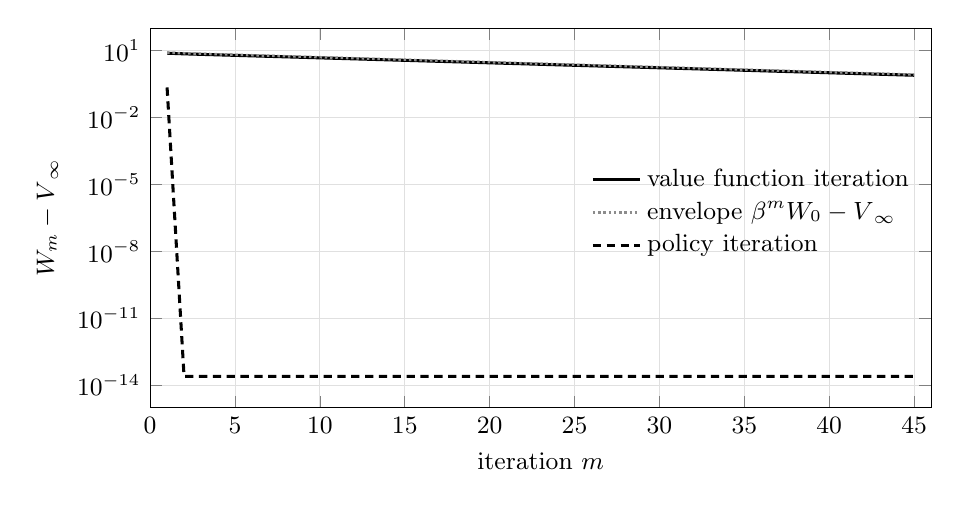
\begin{tikzpicture}
	\begin{semilogyaxis}[
			width=11.5cm, height=6.4cm,
			xlabel={iteration $m$},
			ylabel={$\norm{W_m-V}_\infty$},
			xmin=0, xmax=46,
			ymin=1e-15, ymax=1e2,
			ytick={1e-14,1e-11,1e-8,1e-5,1e-2,1e1},
			tick label style={font=\small},
			label style={font=\small},
			legend cell align=left,
			legend style={draw=none, fill=none, font=\small,
					at={(0.99,0.66)}, anchor=north east},
			grid=major,
			grid style={line width=0.3pt, draw=black!12},
		]
		\addplot[line width=1.1pt, mark=none] table[x index=0, y index=2] {
				1 2.2179551349e-01 7.6079193299e+00 7.9675738255e+00
				2 2.4868995752e-14 7.1224199582e+00 7.5691951342e+00
				3 2.4868995752e-14 6.7465506007e+00 7.1907353775e+00
				4 2.4868995752e-14 6.4062691500e+00 6.8311986087e+00
				5 2.4868995752e-14 6.0853967868e+00 6.4896386782e+00
				6 2.4868995752e-14 5.7809940599e+00 6.1651567443e+00
				7 2.4868995752e-14 5.4919241232e+00 5.8568989071e+00
				8 2.4868995752e-14 5.2173248913e+00 5.5640539617e+00
				9 2.4868995752e-14 4.9564580540e+00 5.2858512637e+00
				10 2.4868995752e-14 4.7086350764e+00 5.0215587005e+00
				11 2.4868995752e-14 4.4732033037e+00 4.7704807654e+00
				12 2.4868995752e-14 4.2495431353e+00 4.5319567272e+00
				13 2.4868995752e-14 4.0370659781e+00 4.3053588908e+00
				14 2.4868995752e-14 3.8352126792e+00 4.0900909463e+00
				15 2.4868995752e-14 3.6434520452e+00 3.8855863990e+00
				16 2.4868995752e-14 3.4612794429e+00 3.6913070790e+00
				17 2.4868995752e-14 3.2882154708e+00 3.5067417251e+00
				18 2.4868995752e-14 3.1238046972e+00 3.3314046388e+00
				19 2.4868995752e-14 2.9676144624e+00 3.1648344069e+00
				20 2.4868995752e-14 2.8192337393e+00 3.0065926865e+00
				21 2.4868995752e-14 2.6782720523e+00 2.8562630522e+00
				22 2.4868995752e-14 2.5443584497e+00 2.7134498996e+00
				23 2.4868995752e-14 2.4171405272e+00 2.5777774046e+00
				24 2.4868995752e-14 2.2962835008e+00 2.4488885344e+00
				25 2.4868995752e-14 2.1814693258e+00 2.3264441077e+00
				26 2.4868995752e-14 2.0723958595e+00 2.2101219023e+00
				27 2.4868995752e-14 1.9687760665e+00 2.0996158072e+00
				28 2.4868995752e-14 1.8703372632e+00 1.9946350168e+00
				29 2.4868995752e-14 1.7768204000e+00 1.8949032660e+00
				30 2.4868995752e-14 1.6879793800e+00 1.8001581027e+00
				31 2.4868995752e-14 1.6035804110e+00 1.7101501975e+00
				32 2.4868995752e-14 1.5234013905e+00 1.6246426877e+00
				33 2.4868995752e-14 1.4472313210e+00 1.5434105533e+00
				34 2.4868995752e-14 1.3748697549e+00 1.4662400256e+00
				35 2.4868995752e-14 1.3061262672e+00 1.3929280243e+00
				36 2.4868995752e-14 1.2408199538e+00 1.3232816231e+00
				37 2.4868995752e-14 1.1787789561e+00 1.2571175420e+00
				38 2.4868995752e-14 1.1198400083e+00 1.1942616649e+00
				39 2.4868995752e-14 1.0638480079e+00 1.1345485816e+00
				40 2.4868995752e-14 1.0106556075e+00 1.0778211525e+00
				41 2.4868995752e-14 9.6012282713e-01 1.0239300949e+00
				42 2.4868995752e-14 9.1211668577e-01 9.7273359016e-01
				43 2.4868995752e-14 8.6651085148e-01 9.2409691066e-01
				44 2.4868995752e-14 8.2318530891e-01 8.7789206512e-01
				45 2.4868995752e-14 7.8202604346e-01 8.3399746187e-01
			};
		\addlegendentry{value function iteration}
		\addplot[line width=0.9pt, mark=none, black!45, densely dotted] table[x index=0, y index=3] {
				1 2.2179551349e-01 7.6079193299e+00 7.9675738255e+00
				2 2.4868995752e-14 7.1224199582e+00 7.5691951342e+00
				3 2.4868995752e-14 6.7465506007e+00 7.1907353775e+00
				4 2.4868995752e-14 6.4062691500e+00 6.8311986087e+00
				5 2.4868995752e-14 6.0853967868e+00 6.4896386782e+00
				6 2.4868995752e-14 5.7809940599e+00 6.1651567443e+00
				7 2.4868995752e-14 5.4919241232e+00 5.8568989071e+00
				8 2.4868995752e-14 5.2173248913e+00 5.5640539617e+00
				9 2.4868995752e-14 4.9564580540e+00 5.2858512637e+00
				10 2.4868995752e-14 4.7086350764e+00 5.0215587005e+00
				11 2.4868995752e-14 4.4732033037e+00 4.7704807654e+00
				12 2.4868995752e-14 4.2495431353e+00 4.5319567272e+00
				13 2.4868995752e-14 4.0370659781e+00 4.3053588908e+00
				14 2.4868995752e-14 3.8352126792e+00 4.0900909463e+00
				15 2.4868995752e-14 3.6434520452e+00 3.8855863990e+00
				16 2.4868995752e-14 3.4612794429e+00 3.6913070790e+00
				17 2.4868995752e-14 3.2882154708e+00 3.5067417251e+00
				18 2.4868995752e-14 3.1238046972e+00 3.3314046388e+00
				19 2.4868995752e-14 2.9676144624e+00 3.1648344069e+00
				20 2.4868995752e-14 2.8192337393e+00 3.0065926865e+00
				21 2.4868995752e-14 2.6782720523e+00 2.8562630522e+00
				22 2.4868995752e-14 2.5443584497e+00 2.7134498996e+00
				23 2.4868995752e-14 2.4171405272e+00 2.5777774046e+00
				24 2.4868995752e-14 2.2962835008e+00 2.4488885344e+00
				25 2.4868995752e-14 2.1814693258e+00 2.3264441077e+00
				26 2.4868995752e-14 2.0723958595e+00 2.2101219023e+00
				27 2.4868995752e-14 1.9687760665e+00 2.0996158072e+00
				28 2.4868995752e-14 1.8703372632e+00 1.9946350168e+00
				29 2.4868995752e-14 1.7768204000e+00 1.8949032660e+00
				30 2.4868995752e-14 1.6879793800e+00 1.8001581027e+00
				31 2.4868995752e-14 1.6035804110e+00 1.7101501975e+00
				32 2.4868995752e-14 1.5234013905e+00 1.6246426877e+00
				33 2.4868995752e-14 1.4472313210e+00 1.5434105533e+00
				34 2.4868995752e-14 1.3748697549e+00 1.4662400256e+00
				35 2.4868995752e-14 1.3061262672e+00 1.3929280243e+00
				36 2.4868995752e-14 1.2408199538e+00 1.3232816231e+00
				37 2.4868995752e-14 1.1787789561e+00 1.2571175420e+00
				38 2.4868995752e-14 1.1198400083e+00 1.1942616649e+00
				39 2.4868995752e-14 1.0638480079e+00 1.1345485816e+00
				40 2.4868995752e-14 1.0106556075e+00 1.0778211525e+00
				41 2.4868995752e-14 9.6012282713e-01 1.0239300949e+00
				42 2.4868995752e-14 9.1211668577e-01 9.7273359016e-01
				43 2.4868995752e-14 8.6651085148e-01 9.2409691066e-01
				44 2.4868995752e-14 8.2318530891e-01 8.7789206512e-01
				45 2.4868995752e-14 7.8202604346e-01 8.3399746187e-01
			};
		\addlegendentry{envelope $\beta^{m}\norm{W_0-V}_\infty$}
		\addplot[line width=1.1pt, mark=none, densely dashed] table[x index=0, y index=1] {
				1 2.2179551349e-01 7.6079193299e+00 7.9675738255e+00
				2 2.4868995752e-14 7.1224199582e+00 7.5691951342e+00
				3 2.4868995752e-14 6.7465506007e+00 7.1907353775e+00
				4 2.4868995752e-14 6.4062691500e+00 6.8311986087e+00
				5 2.4868995752e-14 6.0853967868e+00 6.4896386782e+00
				6 2.4868995752e-14 5.7809940599e+00 6.1651567443e+00
				7 2.4868995752e-14 5.4919241232e+00 5.8568989071e+00
				8 2.4868995752e-14 5.2173248913e+00 5.5640539617e+00
				9 2.4868995752e-14 4.9564580540e+00 5.2858512637e+00
				10 2.4868995752e-14 4.7086350764e+00 5.0215587005e+00
				11 2.4868995752e-14 4.4732033037e+00 4.7704807654e+00
				12 2.4868995752e-14 4.2495431353e+00 4.5319567272e+00
				13 2.4868995752e-14 4.0370659781e+00 4.3053588908e+00
				14 2.4868995752e-14 3.8352126792e+00 4.0900909463e+00
				15 2.4868995752e-14 3.6434520452e+00 3.8855863990e+00
				16 2.4868995752e-14 3.4612794429e+00 3.6913070790e+00
				17 2.4868995752e-14 3.2882154708e+00 3.5067417251e+00
				18 2.4868995752e-14 3.1238046972e+00 3.3314046388e+00
				19 2.4868995752e-14 2.9676144624e+00 3.1648344069e+00
				20 2.4868995752e-14 2.8192337393e+00 3.0065926865e+00
				21 2.4868995752e-14 2.6782720523e+00 2.8562630522e+00
				22 2.4868995752e-14 2.5443584497e+00 2.7134498996e+00
				23 2.4868995752e-14 2.4171405272e+00 2.5777774046e+00
				24 2.4868995752e-14 2.2962835008e+00 2.4488885344e+00
				25 2.4868995752e-14 2.1814693258e+00 2.3264441077e+00
				26 2.4868995752e-14 2.0723958595e+00 2.2101219023e+00
				27 2.4868995752e-14 1.9687760665e+00 2.0996158072e+00
				28 2.4868995752e-14 1.8703372632e+00 1.9946350168e+00
				29 2.4868995752e-14 1.7768204000e+00 1.8949032660e+00
				30 2.4868995752e-14 1.6879793800e+00 1.8001581027e+00
				31 2.4868995752e-14 1.6035804110e+00 1.7101501975e+00
				32 2.4868995752e-14 1.5234013905e+00 1.6246426877e+00
				33 2.4868995752e-14 1.4472313210e+00 1.5434105533e+00
				34 2.4868995752e-14 1.3748697549e+00 1.4662400256e+00
				35 2.4868995752e-14 1.3061262672e+00 1.3929280243e+00
				36 2.4868995752e-14 1.2408199538e+00 1.3232816231e+00
				37 2.4868995752e-14 1.1787789561e+00 1.2571175420e+00
				38 2.4868995752e-14 1.1198400083e+00 1.1942616649e+00
				39 2.4868995752e-14 1.0638480079e+00 1.1345485816e+00
				40 2.4868995752e-14 1.0106556075e+00 1.0778211525e+00
				41 2.4868995752e-14 9.6012282713e-01 1.0239300949e+00
				42 2.4868995752e-14 9.1211668577e-01 9.7273359016e-01
				43 2.4868995752e-14 8.6651085148e-01 9.2409691066e-01
				44 2.4868995752e-14 8.2318530891e-01 8.7789206512e-01
				45 2.4868995752e-14 7.8202604346e-01 8.3399746187e-01
			};
		\addlegendentry{policy iteration}
	\end{semilogyaxis}
\end{tikzpicture}

	\caption[Policy iteration against value function iteration]{%
		Distance to the optimal value function under the two algorithms, started
		from the value $W_0$ of the same stationary policy on a randomly generated
		Markov decision problem with $40$ states, $8$ actions and $\beta=0.95$.
		The vertical axis is logarithmic. The dashed curve lies below the solid
		one at every step, which is
		\autoref{thm:policy-iteration}(ii); it flattens at $2.5\times10^{-14}$
		because the linear solve in \eqref{eq:policy-evaluation} returns the exact
		value of the optimal policy up to rounding, so the remaining error is the
		conditioning of $I-\beta P_{h}$ and not the contraction.}
	\label{fig:pi-vs-vi}
\end{figure}

\section{First-Order Conditions and the Envelope Formula}\label{sec:dyn-foc}

Contraction gives existence, uniqueness and an algorithm, but no
characterisation. Characterisation comes from differentiating the Bellman
equation, and that requires knowing that $V$ is differentiable --- which is a
conclusion, not an assumption, since $V$ is defined as a supremum.

\begin{lemma}[Supergradients of a concave function]\label{lem:supergradient}
	Let $V\colon X\to\R$ be concave on a convex $X\subseteq\R^{n}$ and let
	$x_0\in\Int X$. Then there exists $p\in\R^{n}$ with
	\begin{equation}\label{eq:supergradient}
		V(x)\leq V(x_0)+\ip{p}{x-x_0}\qquad\text{for every }x\in X,
	\end{equation}
	and $V$ is differentiable at $x_0$ if and only if such a $p$ is unique, in which
	case $p=\nabla V(x_0)$.
\end{lemma}

\begin{proof}
	The hypograph $\hyp V=\{(x,t)\in X\times\R : t\leq V(x)\}$ is convex, by the
	concave analogue of \autoref{prop:convex-epigraph}, and $(x_0,V(x_0))$ is a
	boundary point of it. \autoref{thm:supporting-hyperplane} supplies
	$(a,b)\neq0$ with $\ip{a}{x}+bt\leq\ip{a}{x_0}+bV(x_0)$ for all
	$(x,t)\in\hyp V$. Letting $t\to-\infty$ forces $b\geq0$; and $b=0$ would give
	$\ip{a}{x-x_0}\leq0$ for all $x\in X$ with $a\neq0$, impossible for $x_0$
	interior. Dividing by $b>0$ and setting $p\eqdef-a/b$ gives
	\eqref{eq:supergradient} on taking $t=V(x)$. The equivalence of uniqueness with
	differentiability is \textcite[Thm.~25.1]{rockafellar1970convex}.
\end{proof}

\begin{theorem}[Benveniste--Scheinkman]\label{thm:benveniste-scheinkman}
	Let $X\subseteq\R^{n}$ be convex, $V\colon X\to\R$ concave, and
	$x_0\in\Int X$. Suppose there is a neighbourhood $D\subseteq X$ of $x_0$ and a
	concave function $W\colon D\to\R$, differentiable at $x_0$, with
	\begin{equation}\label{eq:bs-sandwich}
		W(x_0)=V(x_0)\qquad\text{and}\qquad W(x)\leq V(x)\ \text{ for all }x\in D .
	\end{equation}
	Then $V$ is differentiable at $x_0$ and $\nabla V(x_0)=\nabla W(x_0)$.
\end{theorem}

\begin{proof}
	Let $p$ satisfy \eqref{eq:supergradient} for $V$ at $x_0$, which
	\autoref{lem:supergradient} provides. For $x\in D$,
	\[
		W(x)\leq V(x)\leq V(x_0)+\ip{p}{x-x_0}=W(x_0)+\ip{p}{x-x_0},
	\]
	so $p$ is a supergradient of $W$ at $x_0$. But $W$ is differentiable at $x_0$,
	so by \autoref{lem:supergradient} its supergradient there is unique and equals
	$\nabla W(x_0)$; hence $p=\nabla W(x_0)$. Since $p$ was an arbitrary
	supergradient of $V$, the supergradient of $V$ at $x_0$ is unique, and
	\autoref{lem:supergradient} makes $V$ differentiable there with
	$\nabla V(x_0)=\nabla W(x_0)$.
\end{proof}

This is \textcite{benveniste1979differentiability}. Applying it requires
producing a $W$ that is concave on a neighbourhood of $x_0$, differentiable at
$x_0$, equal to $V$ there and dominated by $V$ nearby. In a dynamic programme the
candidate is the value of freezing the control at its optimal value and letting
the state vary, and whether that candidate is admissible depends on how the state
enters the transition. The next theorem is therefore stated for problems written
with the next state as the control, which is the form every application in this
chapter takes.

\begin{assumption}[Next state as control]\label{ass:next-state}
	$X\subseteq\R$ is an interval, the control is the next state, so that
	$g(x,u)=u$ and $\Gamma(x)\subseteq X$, and:
	\begin{enumerate}[(i)]
		\item $r$ is continuously differentiable on $\gph\Gamma$ and $r(\cdot,u)$ is
		      concave for each $u$;
		\item the optimal policy $h$ is single-valued and $h(x)\in\Int\Gamma(x)$ for
		      $x\in\Int X$;
		\item $\Gamma$ expands locally at every $x\in\Int X$: there is a
		      neighbourhood $D$ of $x$ with $h(x)\in\Gamma(z)$ for every $z\in D$.
	\end{enumerate}
\end{assumption}

Hypothesis (iii) is what makes the frozen control feasible at neighbouring
states, and it holds in each application below: in the cake problem
$\Gamma(w)=[0,w]$ and $h(w)=\beta w<w$; in the growth model
$\Gamma(k)=[0,f(k)+(1-\delta)k]$ and $h(k)$ is interior.

\begin{theorem}[Euler equation and envelope formula]\label{thm:euler-envelope}
	Let \autoref{ass:dyn} and \autoref{ass:next-state} hold and let $V$ be concave.
	Then at every $x\in\Int X$ the optimal control $u^{\ast}=h(x)$ satisfies the
	\dfnas{first-order condition, dynamic}{first-order condition}
	\begin{equation}\label{eq:dyn-foc}
		\frac{\partial r}{\partial u}(x,u^{\ast})+\beta V'(u^{\ast})=0,
	\end{equation}
	and $V$ is differentiable at $x$ with the \dfnas{envelope
		formula}{envelope formula}
	\begin{equation}\label{eq:dyn-envelope}
		V'(x)=\frac{\partial r}{\partial x}(x,u^{\ast}) .
	\end{equation}
\end{theorem}

\begin{proof}
	\emph{Differentiability and \eqref{eq:dyn-envelope}.} Fix $x\in\Int X$, write
	$u^{\ast}=h(x)$, and let $D$ be the neighbourhood supplied by
	\autoref{ass:next-state}(iii). Define
	\[
		W(z)\eqdef r(z,u^{\ast})+\beta V(u^{\ast}),\qquad z\in D .
	\]
	The second term is a constant, so $W$ is concave on $D$ by
	\autoref{ass:next-state}(i) and differentiable at $x$ with
	$W'(x)=r_x(x,u^{\ast})$; here is where writing the control as the next state
	pays, since the continuation value does not depend on $z$ and no
	differentiability of $V$ is presupposed. Feasibility of $u^{\ast}$ at $z$ gives
	$W(z)\leq V(z)$ on $D$, and optimality of $u^{\ast}$ at $x$ gives $W(x)=V(x)$.
	\autoref{thm:benveniste-scheinkman} now yields differentiability of $V$ at $x$
	and $V'(x)=W'(x)=r_x(x,u^{\ast})$.

	\emph{The first-order condition.} The preceding paragraph applies at every
	interior point, in particular at $u^{\ast}\in\Int\Gamma(x)\subseteq\Int X$, so
	$V$ is differentiable at $u^{\ast}$. The map
	$u\mapsto r(x,u)+\beta V(u)$ is therefore differentiable at its interior
	maximiser $u^{\ast}$, and \autoref{thm:fermat} gives \eqref{eq:dyn-foc}.
\end{proof}

\begin{remark}[The general transition]\label{rem:general-transition}
	When the transition is a genuine function $g(x,u)$ of both arguments, the same
	construction gives
	$W(z)=r(z,u^{\ast})+\beta V\bigl(g(z,u^{\ast})\bigr)$, whose differentiability
	at $x$ requires $V$ to be differentiable at $g(x,u^{\ast})$ --- which is what
	was to be proved. The circularity is not an artefact: differentiability of $V$
	must then be obtained from the whole optimal plan rather than from one period,
	by taking
	\[
		W(z)\eqdef\sum_{t\geq0}\beta^{t}r\bigl(z_t,u^{\ast}_t\bigr),
		\qquad z_0=z,\quad z_{t+1}=g(z_t,u^{\ast}_t),
	\]
	with $(u^{\ast}_t)$ the optimal control sequence from $x$. This $W$ is concave
	whenever each $g(\cdot,u)$ is affine and each $r(\cdot,u)$ concave, and
	differentiable at $x$ under a bound $\sup\abs{g_x}\leq G$ with $\beta G<1$ that
	makes the differentiated series converge. Every problem treated below is
	already in the form of \autoref{ass:next-state}, and any problem with
	$g(x,\cdot)$ invertible can be put in that form by taking the next state as the
	control, so the general construction is not needed here. It is set out in
	\textcite[Sec.~4.3]{stokey1989recursive}.
\end{remark}

\begin{remark}[The derivation by differentiating the policy]\label{rem:envelope-direct}
	The derivation on \autocite[slide 18]{fukuda2026dynamic} differentiates
	$V(x)=r(x,h(x))+\beta V(h(x))$ directly, obtaining
	\[
		V'(x)=\underbrace{\Bigl[r_u\bigl(x,h(x)\bigr)+\beta V'\bigl(h(x)\bigr)\Bigr]}_{=0\ \text{by }\eqref{eq:dyn-foc}}h'(x)
		+r_x\bigl(x,h(x)\bigr),
	\]
	so that the term in $h'$ drops out and \eqref{eq:dyn-envelope} remains. The
	computation is right in content and presupposes what is at issue: that $V$ and
	$h$ are differentiable. \autoref{thm:benveniste-scheinkman} establishes the
	conclusion without differentiating $h$ at all, and therefore without assuming
	the policy is smooth --- which it need not be, since
	\autoref{thm:bellman-contraction} delivers only upper hemicontinuity.
\end{remark}

\begin{corollary}[Euler equation for a depletable stock]\label{cor:euler}
	Let \autoref{ass:dyn} and \autoref{ass:next-state} hold with
	$X=[0,\infty)$, $\Gamma(x)=[0,x]$ and $r(x,u)=\tilde r(x-u)$ for a
	continuously differentiable, strictly increasing and concave $\tilde r$, so
	that the state is a stock, the control is the stock carried forward and
	$c\eqdef x-u$ is the amount consumed. Let $V$ be concave. Then along an
	interior optimal path
	\begin{equation}\label{eq:euler-dyn}
		\tilde r'(c_t)=\beta\,\tilde r'(c_{t+1})\qquad\text{for every }t .
	\end{equation}
\end{corollary}

\begin{proof}
	Here $r_u(x,u)=-\tilde r'(x-u)$ and $r_x(x,u)=\tilde r'(x-u)$, so
	\eqref{eq:dyn-foc} reads $\tilde r'(c_t)=\beta V'(x_{t+1})$ and
	\eqref{eq:dyn-envelope} reads $V'(x_t)=\tilde r'(c_t)$. Substituting the
	envelope formula at $t+1$ into the first-order condition at $t$,
	\[
		\tilde r'(c_t)=\beta V'(x_{t+1})
		\overset{\text{envelope}}{=}\beta\,\tilde r'(c_{t+1}),
	\]
	which is \eqref{eq:euler-dyn}.
\end{proof}

The chain in the proof --- first-order condition, envelope, first-order condition
--- is the standard route from a Bellman equation to an Euler equation, and it
eliminates the unknown $V'$ entirely: the Euler equation involves only
primitives \autocite[slide 32]{fukuda2026dynamic}. Its economic reading is a
no-arbitrage condition along the optimal path. Consuming $\Delta$ less today
costs $\tilde r'(c_t)\Delta$ in current utility and returns
$\beta\tilde r'(c_{t+1})\Delta$ in discounted utility tomorrow; at an optimum the
two are equal, and the equality is precisely the first-order condition of the
perturbed problem in $\Delta$ at $\Delta=0$.

\section{The Cake-Eating Problem}\label{sec:dyn-cake}

\paragraph{Problem.} An agent endowed with a cake of size $w_0>0$ chooses
consumption $(c_t)_{t\geq0}$ to maximise $\sum_{t\geq0}\beta^{t}\log c_t$ subject
to $w_{t+1}=w_t-c_t$ and $c_t\geq0$, $w_t\geq0$.

There are two ways to assign the state and the control, and they are not
computationally equivalent \autocite[slides 21--22]{fukuda2026dynamic}. Taking
the control to be consumption gives
$V(w)=\max_{c\in[0,w]}\{\log c+\beta V(w-c)\}$, in which $w-c$ generally falls
between grid points and must be interpolated. Taking the control to be
\emph{tomorrow's cake} gives
\begin{equation}\label{eq:cake-bellman}
	V(w)=\max_{w'\in[0,w]}\ \bigl\{\log(w-w')+\beta V(w')\bigr\},
\end{equation}
in which the transition is the identity on the grid. The second formulation is
the one implemented.

\begin{proposition}[Closed form]\label{prop:cake-solution}
	The cake-eating problem has value function and policy
	\begin{equation}\label{eq:cake-solution}
		V(w)=\frac{\log(1-\beta)}{1-\beta}+\frac{\beta\log\beta}{(1-\beta)^{2}}
		+\frac{\log w}{1-\beta},
		\qquad
		h(w)=(1-\beta)w,
	\end{equation}
	so that $c_t=(1-\beta)\beta^{t}w_0$ and $w_{t+1}=\beta w_t$.
\end{proposition}

\begin{proof}
	The first two steps construct a candidate; the third proves it is the value
	function, and neither of the first two is used in that proof.

	\emph{From the Euler equation.} \autoref{cor:euler} with
	$\tilde r=\log$ gives $1/c_t=\beta/c_{t+1}$, that is $c_{t+1}=\beta c_t$, hence
	$c_\tau=\beta^{\tau-t}c_t$. Imposing exhaustion,
	$w_t=\sum_{\tau\geq t}c_\tau$ --- provisionally, since $\lim_tw_t=0$ is at this
	stage a conjecture about the optimal path rather than a consequence of anything
	proved --- gives
	\[
		w_t=\sum_{\tau=t}^{\infty}\beta^{\tau-t}c_t=\frac{c_t}{1-\beta},
		\qquad\text{so}\qquad c_t=(1-\beta)w_t,
	\]
	which is the stated policy, and then $w_{t+1}=w_t-c_t=\beta w_t$ and
	$c_t=(1-\beta)\beta^{t}w_0$.

	\emph{Value.} Substituting the optimal path into the objective,
	\begin{align*}
		V(w_0) & =\sum_{t=0}^{\infty}\beta^{t}\log\bigl((1-\beta)\beta^{t}w_0\bigr)
		=\log(1-\beta)\sum_{t\geq0}\beta^{t}
		+\log\beta\sum_{t\geq0}t\beta^{t}
		+\log w_0\sum_{t\geq0}\beta^{t}                                            \\
		       & =\frac{\log(1-\beta)}{1-\beta}+\frac{\beta\log\beta}{(1-\beta)^{2}}
		+\frac{\log w_0}{1-\beta},
	\end{align*}
	using $\sum_{t\geq0}\beta^{t}=1/(1-\beta)$ and
	\[
		\sum_{t\geq0}t\beta^{t}=\beta\sum_{t\geq0}t\beta^{t-1}
		=\beta\deriv{}{\beta}\sum_{t\geq0}\beta^{t}
		=\beta\deriv{}{\beta}\frac{1}{1-\beta}=\frac{\beta}{(1-\beta)^{2}},
	\]
	the term-by-term differentiation being legitimate on $\abs{\beta}<1$, where the
	power series converges uniformly on compact subsets.

	\emph{Verification.} Write $V(w)=A+B\log w$ with $B=1/(1-\beta)$ and $A$ as in
	\eqref{eq:cake-solution}. The objective in \eqref{eq:cake-bellman} is strictly
	concave in $w'$ on $(0,w)$ and tends to $-\infty$ at both endpoints, so its
	unique maximiser is interior and solves
	$1/(w-w')=\beta B/w'$, that is $w'=\beta Bw/(1+\beta B)=\beta w$ since
	$\beta B=\beta/(1-\beta)$ and $1+\beta B=1/(1-\beta)$. Substituting back,
	\[
		\log\bigl((1-\beta)w\bigr)+\beta\bigl(A+B\log(\beta w)\bigr)
		=\underbrace{\log(1-\beta)+\beta A+\beta B\log\beta}_{=A}
		+\underbrace{(1+\beta B)}_{=B}\log w,
	\]
	the first bracket equalling $A$ because $A(1-\beta)=\log(1-\beta)+\beta\log\beta/(1-\beta)$
	by \eqref{eq:cake-solution}. Hence $TV=V$. Optimality of the associated plan
	follows from \eqref{eq:value-unrolled}: along it $w_m=\beta^{m}w_0$, so
	$\beta^{m}V(w_m)=\beta^{m}(A+B\log w_0)+mB\beta^{m}\log\beta\to0$, and the
	transversality condition of \autoref{rem:transversality} holds even though
	\autoref{ass:dyn}(iii) fails.
\end{proof}

The eaten fraction $1-\beta$ is independent of the cake size --- a consequence of
the homotheticity of $\log$ utility, under which the problem scales --- and
independent of time, which is stationarity. The value function inherits the
logarithm from the return function, which is why the guess $A+B\log w$ works and
why it would fail for a return function outside the CRRA class.

\begin{remark}[What the numerical solution adds]\label{rem:cake-numerics}
	\path{DP_cake_eating.m} solves \eqref{eq:cake-bellman} by value function
	iteration on a uniform grid of $2000$ points from $0.001$ to $w_0=1$ with
	$\beta=0.85$, starting from $W_0\equiv0$ and stopping when successive iterates
	differ by less than $10^{-16}$ in the supremum norm
	\autocite[slides 23--30]{fukuda2026dynamic};
	\path{DP_cake_eating_CRRA.m} repeats it for CRRA utility and
	\path{DP_cake_eating_plot_iterations.m} displays the iterates $W_m$ converging
	to $V$. Run as supplied on \textsc{Matlab} R2025b, the first reports
	convergence after $279$ iterations in $1.04$ seconds, the second after $199$,
	the third in $0.11$ seconds. The lower endpoint is not zero because
	$\log0=-\infty$; the truncation discretises the state space rather than
	approximating the economics. Because \eqref{eq:cake-solution} is available in
	closed form, the whole discrepancy is numerical error and can be located.

	Measured against \eqref{eq:cake-solution}, the computed value function is off
	by $12.06$ at $w=0.001$, by at most $0.33$ on $w\geq0.1$ and by $0.033$ at
	$w=1$: the error lives at the bottom of the grid, where the truncation bites
	and $\log$ is unbounded. The computed policy differs from $(1-\beta)w$ by at
	most $0.00122$ at every node above the first, which is under three grid
	spacings of $5.0\times10^{-4}$. \autoref{fig:vfi-error} plots both errors.

	At the first node the reported consumption is $-0.999$, an artefact of the line
	\[
		\verb|consumption(consumption<=0)=0.1^16|.
	\]
	At $w=0.001$ no grid choice of $w'$
	leaves positive consumption, so every entry of that row of the consumption
	matrix is the sentinel $10^{-16}$; the entries of $\log c+\beta W$ then differ
	only through $\beta W(w')$, which is largest at $w'=1$, and the row maximum is
	decided by the continuation value alone. The plotted range
	$[0,1.05(1-\beta)]$ keeps this out of the figure.

	Replacing the sentinel by $-\infty$ removes that artefact and creates a worse
	one. The lowest node then has value $-\infty$; the second node's only feasible
	continuation is the lowest node, so it too becomes $-\infty$, and by induction
	every node does. The truncated state space $[0.001,1]$ is not invariant under
	the optimal policy $w'=\beta w$, and a grid bounded away from zero cannot
	represent the tail of the optimal path --- which is what the program's own
	comment about \verb|num_period| records. The repair has to supply a boundary
	condition as well: set the infeasible cells to $-\infty$ and hold the lowest
	node at the analytic value $V(0.001)=-64.8388$ from \eqref{eq:cake-solution}.
	Run that way in \textsc{Matlab} R2025b, the recursion converges in $51$
	iterations rather than $279$, reports consumption $0$ at the lowest node, and
	improves every error measure: the value error is $0.0238$ rather than $0.325$
	on $w\geq0.1$ and $0.00236$ rather than $0.0335$ at $w=1$, and the policy
	error is at most $5.75\times10^{-4}$ rather than $1.22\times10^{-3}$, that is
	one grid spacing rather than three. The dashed curves of
	\autoref{fig:vfi-error} are this variant.

	The four sources of error in \eqref{eq:cake-bellman} separate cleanly, which
	is why the exercise is instructive:
	\begin{itemize}
		\item \emph{iteration error}, bounded by \eqref{eq:vfi-error}, and
		      measurable here because the analytic $V$ is known --- the observed
		      ratio of successive errors is $\exp(-0.16252)=\beta$ to five
		      decimals;
		\item \emph{discretisation error}, from restricting $w'$ to the grid, of
		      order the spacing $5.0\times10^{-4}$, which is what the policy error
		      attains;
		\item \emph{truncation error}, from replacing the state space $(0,1]$ by
		      $[0.001,1]$, which is what the boundary condition addresses and
		      which is the largest term at the bottom of the grid;
		\item \emph{interpolation and quadrature error}, both zero here, since the
		      choice set is the grid itself and the problem is deterministic.
	\end{itemize}
	In \path{Lucas_Tree_DP.m} the last item is not zero: the conditional
	expectation is a $500$-draw Monte Carlo average and the continuation value is
	a spline interpolant, and the residual $0.0103\%$ against the closed-form
	price $\beta y/(1-\beta)$ is dominated by those two.

	The stopping rule is also not the one analysed in \autoref{rem:vfi}. Here
	$\norm{W_1-W_0}_\infty=36.84$, so \eqref{eq:vfi-error} gives
	$\norm{W_m-W_{m-1}}_\infty<10^{-16}$ by $m=261$. The computed value function
	reaches $-52.78$ at the lowest node, where consecutive doubles are
	$7.1\times10^{-15}$ apart --- far above the tolerance. From about iteration
	$240$ the computed increment is quantised at one unit in the last place, and
	the test can succeed only when the iteration lands on an exact floating-point
	fixed point. Reimplementing the same recursion with the continuation values
	added by broadcasting rather than by the matrix product
	\verb|beta*ones(dimW,1)*V| terminates at $255$ iterations instead of $279$. A
	tolerance below the machine resolution of the value scale gives the
	termination decision to the rounding rather than to the contraction modulus;
	a tolerance of, say, $10^{-10}$ would be governed by \eqref{eq:vfi-error} and
	would stop at a certified accuracy.
\end{remark}

\begin{figure}[htbp]
	\centering
	\input{Figures/vfi-error.tex}
	\caption[Discretisation error of the cake-eating value function iteration]{%
		Absolute error of the converged value function iteration in
		\texttt{DP\_cake\_eating.m} against the closed form
		\eqref{eq:cake-solution}, and of the induced policy against
		$(1-\beta)w$, on the program's own grid with $\beta=0.85$. Solid and
		light-solid curves use the sentinel $10^{-16}$ of the supplied code;
		dashed and dotted curves use $-\infty$ on infeasible pairs together with
		the analytic value at the lowest node. Both axes are logarithmic and the
		first node is omitted. The error in the value function is a boundary
		phenomenon under either encoding, falling by more than two orders of
		magnitude between $w=0.0015$ and $w=1$; the boundary condition lowers it
		by a further factor of about fourteen at the top of the grid, and halves
		the policy error to one grid spacing.}
	\label{fig:vfi-error}
\end{figure}


\section{The Ramsey Growth Model}\label{sec:dyn-ramsey}

\paragraph{Problem.} A planner chooses consumption to maximise
$\sum_{t\geq0}\beta^{t}u(c_t)$ subject to
\begin{equation}\label{eq:ramsey-constraint}
	k_{t+1}=f(k_t)+(1-\delta)k_t-c_t,
	\qquad f(k)=Ak^{\alpha},\ \alpha\in(0,1),\ A>0,\ \delta\in(0,1],
\end{equation}
with $k_0>0$ given, $c_t\geq0$ and $k_t\geq0$; $u$ is strictly increasing,
strictly concave and continuously differentiable on $(0,\infty)$. In recursive
form, writing $\varphi(k)\eqdef f(k)+(1-\delta)k$ for the resources available at
$k$,
\begin{equation}\label{eq:ramsey-bellman}
	V(k)=\max_{k'\in[0,\varphi(k)]}
	\bigl\{u\bigl(\varphi(k)-k'\bigr)+\beta V(k')\bigr\}.
\end{equation}

The theory of \autoref{sec:dyn-contraction} does not apply to
\eqref{eq:ramsey-bellman} as written: the state space $[0,\infty)$ is unbounded
and $u$ need not be bounded on the feasible consumption set, so
\autoref{ass:dyn} fails on both counts. Both are repaired before the Euler
equation is derived.

\begin{lemma}[Standing hypotheses for the growth model]\label{lem:ramsey-standing}
	Put $k_{g}\eqdef(A/\delta)^{1/(1-\alpha)}$, the unique positive solution of
	$f(k)=\delta k$, and $\bar k\eqdef\max\{k_0,k_{g}\}$. On $X\eqdef[0,\bar k]$
	with $\Gamma(k)\eqdef[0,\varphi(k)]$ and $g(k,k')\eqdef k'$:
	\begin{enumerate}[(i)]
		\item $X$ is invariant, that is $\Gamma(k)\subseteq X$ for every $k\in X$;
		\item $\Gamma$ is non-empty- and compact-valued and continuous, and $g$ is
		      continuous;
		\item if $u$ extends to a real-valued continuous function on $[0,\infty)$,
		      then $r(k,k')\eqdef u(\varphi(k)-k')$ is continuous and bounded on
		      $\gph\Gamma$.
	\end{enumerate}
	Under (iii), \autoref{ass:dyn} holds on $X$ for every $\beta\in(0,1)$.
\end{lemma}

\begin{proof}
	(i) $\varphi$ is strictly increasing, so
	$\max_{k\in X}\varphi(k)=\varphi(\bar k)$, and
	$\varphi(\bar k)\leq\bar k$ is equivalent to $A\bar k^{\alpha}\leq\delta\bar k$,
	that is to $\bar k\geq k_{g}$, which holds by construction. Hence
	$\Gamma(k)\subseteq[0,\varphi(\bar k)]\subseteq[0,\bar k]=X$.

	(ii) $\Gamma(k)$ contains $0$ and is a compact interval. For upper
	hemicontinuity, if $k_j\to k$ and $u_j\in\Gamma(k_j)$ with $u_j\to u$, then
	$0\leq u\leq\lim\varphi(k_j)=\varphi(k)$ by continuity of $\varphi$. For lower
	hemicontinuity, given $u\in\Gamma(k)$ and $k_j\to k$, set
	$u_j\eqdef\min\{u,\varphi(k_j)\}\in\Gamma(k_j)$; then $u_j\to u$, again by
	continuity of $\varphi$. Continuity of $g$ is immediate.

	(iii) On $\gph\Gamma$ the consumption $c=\varphi(k)-k'$ ranges over the
	compact interval $[0,\varphi(\bar k)]$, on which the continuous $u$ is bounded
	by \autoref{cor:weierstrass-continuous}; and $r$ is continuous as a
	composition of continuous maps.
\end{proof}

\begin{remark}[Utility unbounded at zero consumption]\label{rem:ramsey-unbounded}
	Hypothesis (iii) is where $u=\log$ and CRRA with $\gamma\geq1$ fail. Zero
	consumption is feasible at every $k$, and $u(0^{+})=-\infty$, so $r$ is
	unbounded below and \autoref{ass:dyn}(iii) holds on no state space that
	permits $c=0$: the failure is in the control, not in the state, and confining
	$k$ to a compact interval does not remove it. Two repairs are available.

	\emph{A consumption floor.} Fix $k_{\min}\in(0,k_{g})$, so that
	$\varphi(k_{\min})>k_{\min}$, and $\varepsilon\in(0,\varphi(k_{\min})-k_{\min})$.
	On $X_\varepsilon\eqdef[k_{\min},\bar k]$ with
	$\Gamma_\varepsilon(k)\eqdef[k_{\min},\varphi(k)-\varepsilon]$ the argument of
	\autoref{lem:ramsey-standing} goes through unchanged, and consumption now
	ranges over $[\varepsilon,\varphi(\bar k)-k_{\min}]$, a compact subinterval of
	$(0,\infty)$ on which $u$ is bounded. This is a different problem, and whether
	it has the same solution has to be checked rather than assumed. For $u=\log$
	and $\delta=1$ it can be: the closed-form policy $k'=\alpha\beta Ak^{\alpha}$
	leaves consumption $c=(1-\alpha\beta)Ak^{\alpha}\geq(1-\alpha\beta)Ak_{\min}^{\alpha}$,
	so any $\varepsilon$ below that bound leaves the floor slack and the optimum
	unchanged.

	\emph{A weighted norm.} Alternatively keep $\Gamma$ and replace the supremum
	norm by $\norm{\cdot}_{\phi}$ of \autoref{thm:weighted-contraction} with a
	$\phi$ growing at the rate at which $u$ diverges. Verifying the weighted
	discounting condition (ii) of that theorem for the growth model is carried out
	in \textcite[Ch.~4]{stokey1989recursive} and is not reproduced here.
\end{remark}

\begin{proposition}[Euler equation and steady state]\label{prop:ramsey}
	Assume \autoref{ass:dyn} holds on the state space $X$, as it does under
	\autoref{lem:ramsey-standing}(iii) or under the consumption floor of
	\autoref{rem:ramsey-unbounded}, and assume the optimal policy $h$ is
	single-valued with $h(k)\in\Int\Gamma(k)$ for every $k\in\Int X$, so that
	consumption is strictly positive along the optimal path. Then
	\begin{equation}\label{eq:ramsey-euler}
		u'(c_t)=\beta\,u'(c_{t+1})\bigl(f'(k_{t+1})+1-\delta\bigr),
	\end{equation}
	and the unique interior steady state $(k^{\ast},c^{\ast})$ with
	$c_t\equiv c^{\ast}$, $k_t\equiv k^{\ast}$ is
	\begin{equation}\label{eq:ramsey-steady-state}
		k^{\ast}=\left(\frac{\alpha A}{\beta^{-1}-(1-\delta)}\right)^{\frac{1}{1-\alpha}},
		\qquad
		c^{\ast}=A(k^{\ast})^{\alpha}-\delta k^{\ast}.
	\end{equation}
\end{proposition}

\begin{proof}
	Apply \autoref{thm:euler-envelope} with state $k$, control $k'$ and
	$r(k,k')=u(\varphi(k)-k')$, which is of the form required by
	\autoref{ass:next-state}: $r(\cdot,k')$ is concave as the composition of the
	concave increasing $u$ with the concave $\varphi(\cdot)-k'$; part (ii) of that
	assumption is the interiority hypothesis; and $\Gamma$ expands locally at
	every $k\in\Int X$ because $\varphi$ is increasing and continuous, so
	$h(k)<\varphi(k)$ implies $h(k)<\varphi(z)$ for all $z$ in a neighbourhood
	of $k$. Then
	$r_{k'}=-u'(c)$, so \eqref{eq:dyn-foc} gives
	\begin{equation}\label{eq:ramsey-foc}
		u'(c_t)=\beta V'(k_{t+1});
	\end{equation}
	and $r_k=u'(c)\bigl(f'(k)+1-\delta\bigr)$, so
	\eqref{eq:dyn-envelope} gives
	\begin{equation}\label{eq:ramsey-envelope}
		V'(k_t)=u'(c_t)\bigl(f'(k_t)+1-\delta\bigr).
	\end{equation}
	Substituting \eqref{eq:ramsey-envelope} at $t+1$ into \eqref{eq:ramsey-foc}
	yields \eqref{eq:ramsey-euler}. Concavity of $V$, required by
	\autoref{thm:euler-envelope}, follows from concavity of $u$ and of the
	constraint set: \autoref{prop:value-concave} applies to each iterate $T^{m}W_0$
	started from a concave $W_0$, and \autoref{thm:bellman-contraction} makes the
	uniform limit $V$ concave, uniform limits preserving the inequality in
	\autoref{def:convex-function}.

	At a steady state, $c_t=c_{t+1}$ cancels $u'$ from \eqref{eq:ramsey-euler},
	leaving $1=\beta\bigl(f'(k^{\ast})+1-\delta\bigr)$, that is
	$\alpha A(k^{\ast})^{\alpha-1}=\beta^{-1}-(1-\delta)$, which rearranges to the
	first half of \eqref{eq:ramsey-steady-state}; the exponent
	$1/(1-\alpha)$ is positive and the right-hand side is positive because
	$\beta^{-1}>1\geq1-\delta$, so $k^{\ast}$ exists and is unique. Setting
	$k_{t+1}=k_t=k^{\ast}$ in \eqref{eq:ramsey-constraint} gives
	$c^{\ast}=f(k^{\ast})-\delta k^{\ast}$.
\end{proof}

The steady state lies inside the state space of \autoref{lem:ramsey-standing}:
$k^{\ast}<k_{g}$ is equivalent to $\alpha A/R<A/\delta$, that is to
$\alpha\delta<\beta^{-1}-1+\delta$, which holds because $\beta<1$ and
$\alpha<1$. Interiority of the policy, assumed in \autoref{prop:ramsey}, is
delivered by the Inada conditions $u'(0^{+})=+\infty$ and $f'(0^{+})=+\infty$
together with $k_0>0$: with infinite marginal utility at zero consumption no
optimal plan sets $c_t=0$, and with infinite marginal product at zero capital no
optimal plan sets $k_{t+1}=0$. The argument is in
\textcite[Ch.~5]{stokey1989recursive} and is not reproduced here, since it
requires the monotonicity and differentiability results for $V$ that
\autoref{thm:euler-envelope} presupposes.

Equation \eqref{eq:ramsey-euler} is the intertemporal condition of the
one-sector growth model: the marginal utility cost of investing a unit today
equals its discounted marginal utility return, the return being the marginal
product of capital plus the undepreciated remainder. The steady-state condition
$\beta\bigl(f'(k^{\ast})+1-\delta\bigr)=1$ is the modified golden rule: the net
marginal product $f'(k^{\ast})-\delta$ equals the rate of time preference
$\beta^{-1}-1$. Capital is therefore below the golden-rule level that maximises
steady-state consumption, at which $f'(k)=\delta$, and the wedge is impatience.

For comparative statics write $R\eqdef\beta^{-1}-(1-\delta)>0$, so that
$k^{\ast}=(\alpha A/R)^{1/(1-\alpha)}$ and
\[
	\log k^{\ast}=\frac{1}{1-\alpha}\bigl(\log\alpha+\log A-\log R\bigr).
\]
Since $R$ is decreasing in $\beta$ and increasing in $\delta$, and $\alpha$ is
held fixed in both cases, $k^{\ast}$ is increasing in $\beta$, increasing in $A$
with elasticity $1/(1-\alpha)$, and decreasing in $\delta$. The parameter
$\alpha$ is different, because it enters both the level and the exponent:
\begin{equation}\label{eq:ramsey-alpha}
	\pderiv{\log k^{\ast}}{\alpha}
	=\frac{1}{(1-\alpha)^{2}}\log\frac{\alpha A}{R}+\frac{1}{\alpha(1-\alpha)} .
\end{equation}
The second term is positive and the first has the sign of $\alpha A-R$, so
$k^{\ast}$ is increasing in $\alpha$ whenever $\alpha A\geq R$, which is the
empirically relevant configuration --- with $A=1$, $\alpha=0.3$, $\delta=0.1$ and
$\beta=0.95$ one has $R\approx0.153$ and $\alpha A/R\approx1.97$, giving
$\partial\log k^{\ast}/\partial\alpha\approx6.14$. It is not a general property.
Taking $A=0.01$ with the same $\alpha,\delta,\beta$ gives $\alpha A/R\approx0.020$
and $\partial\log k^{\ast}/\partial\alpha\approx-3.26$, so raising the capital
share \emph{lowers} the steady-state stock. The reason is dimensional: $k^{\ast}$
is measured in units in which $A$ is a pure number, and when $A$ is small the
steady-state capital stock is below one, so a larger exponent $1/(1-\alpha)$
pushes it further down. Comparative statics in $\alpha$ are therefore statements
about a particular normalisation of units, not about technology alone.

Unlike \autoref{sec:dyn-cake} the model has no closed form for general $u$ and
$\delta<1$; the exception is $\delta=1$ with $u=\log$, where the policy is
$k'=\alpha\beta\bigl(Ak^{\alpha}\bigr)$. This is why the numerical treatment of
\autocite[slides 37--41]{fukuda2026dynamic} restricts the grid to
$[k_{\min},k_{\max}]$ containing $k^{\ast}$ with $k_{\min}>0$, which is the
consumption-floor construction of \autoref{rem:ramsey-unbounded} in numerical
dress: the grid never offers a next-period capital above the largest node, so
consumption is bounded away from zero at every node. On that compact set the
return
function is bounded, \autoref{ass:dyn} holds, and
\autoref{thm:bellman-contraction} applies as stated. The program
\path{deterministic_Ramsey_growth.m} computes $k^{\ast}$ from
\eqref{eq:ramsey-steady-state} first and then lays $1000$ nodes over
$[0.25k^{\ast},1.75k^{\ast}]$, so the compact set is chosen by the theory rather
than guessed; infeasible pairs $(k,k')$ receive a large penalty in place of an
undefined utility, which is the discrete analogue of the constraint
$c_t\geq0$. Run as supplied it converges in $211$ iterations.

\section{The Lucas Asset-Pricing Model}\label{sec:dyn-lucas}

\paragraph{Environment.} A representative agent in an endowment economy consumes
a single non-storable good produced by a single tree. The endowment
$(y_t)_{t\geq0}$ is Markov, $y_{t+1}=G(y_t,\varepsilon_{t+1})$ with
$(\varepsilon_t)$ i.i.d.\ with distribution $\varphi$; in the numerical
implementation $\log y_{t+1}=\alpha\log y_t+\sigma\varepsilon_{t+1}$ with
$\varepsilon_t$ standard normal. The agent ranks streams by
$\E_0\bigl[\sum_{t\geq0}\beta^{t}u(c_t)\bigr]$ with $u$ of the CRRA form. A share
$\pi_t\in[0,1]$ of the tree, chosen at $t-1$, is the agent's only store of value,
and an ex-dividend claim bought at price $p_t$ entitles the holder to $y_{t+1}$
and to the resale price $p_{t+1}$.

\paragraph{The agent's problem.} With the share as state alongside the endowment,
\begin{equation}\label{eq:lucas-bellman}
	v(\pi,y)=\max_{\pi'}\
	\Bigl\{u\bigl((y+p(y))\pi-p(y)\pi'\bigr)
	+\beta\int v\bigl(\pi',G(y,z)\bigr)\varphi(\diff z)\Bigr\},
\end{equation}
the budget constraint $c+p(y)\pi'\leq(y+p(y))\pi$ binding because $u$ is strictly
increasing. The agent takes the pricing function $p(\cdot)$ as given; the guess
that the price depends on the history only through the current endowment is
verified by the construction below, and is legitimate because the endowment is
Markov.

\begin{theorem}[Consumption-based asset pricing]\label{thm:lucas-pricing}
	In a competitive equilibrium of the Lucas economy the pricing function satisfies
	\begin{equation}\label{eq:lucas-functional}
		p(y)=\beta\int\frac{u'\bigl(G(y,z)\bigr)}{u'(y)}
		\Bigl(G(y,z)+p\bigl(G(y,z)\bigr)\Bigr)\varphi(\diff z),
	\end{equation}
	equivalently, in sequence form,
	\begin{equation}\label{eq:sdf}
		p_t=\E_t\left[\underbrace{\beta\frac{u'(y_{t+1})}{u'(y_t)}}_{\text{stochastic discount factor}}
			\bigl(y_{t+1}+p_{t+1}\bigr)\right].
	\end{equation}
\end{theorem}

\begin{proof}
	The first-order condition of \eqref{eq:lucas-bellman} in $\pi'$ is
	\begin{equation}\label{eq:lucas-foc}
		u'(c)\,p(y)=\beta\int v_1\bigl(\pi',G(y,z)\bigr)\varphi(\diff z),
		\qquad v_1\eqdef\frac{\partial v}{\partial\pi},
	\end{equation}
	the cost in current marginal utility of an extra share equalling its discounted
	expected marginal value. Differentiating \eqref{eq:lucas-bellman} in the state
	$\pi$ with $\pi'$ held at its optimum --- which is legitimate by
	\autoref{thm:benveniste-scheinkman}, $v$ being concave in $\pi$ as the value of
	a concave problem on a convex constraint set --- gives the envelope formula
	\begin{equation}\label{eq:lucas-envelope}
		v_1(\pi,y)=u'(c)\bigl(y+p(y)\bigr),
	\end{equation}
	an extra share being worth the marginal utility of the dividend plus the resale
	value it delivers.

	Two market-clearing conditions pin down the equilibrium. The good is
	non-storable, so $c_t=y_t$; and with a representative agent there is no trade, so
	$\pi_t=1$ for every $t$. Imposing $c=y$ and $\pi=\pi'=1$ and substituting
	\eqref{eq:lucas-envelope} into \eqref{eq:lucas-foc},
	\[
		u'(y)p(y)=\beta\int u'\bigl(G(y,z)\bigr)
		\Bigl(G(y,z)+p\bigl(G(y,z)\bigr)\Bigr)\varphi(\diff z),
	\]
	which is \eqref{eq:lucas-functional} after division by $u'(y)>0$. Rewriting the
	integral as a conditional expectation gives \eqref{eq:sdf}.
\end{proof}

Equation \eqref{eq:sdf} is the central identity of asset pricing: the price of
any claim is the conditional expectation of its payoff weighted by the
\dfnas{stochastic discount factor}{stochastic discount factor}
$m_{t+1}=\beta u'(y_{t+1})/u'(y_t)$. Prices are high for claims that pay off when
consumption is low, because marginal utility is then high; that is the entire
economics, and the equity premium is the statement that the covariance between
$m_{t+1}$ and equity payoffs is empirically far too small to match observed
returns for plausible $\gamma$.

\begin{theorem}[Existence of the pricing function]\label{thm:lucas-contraction}
	Suppose the map
	$y\mapsto\beta\int u'\bigl(G(y,z)\bigr)G(y,z)\,\varphi(\diff z)$
	defines a bounded continuous function $h$ on $\R_+$. Then the operator
	\begin{equation}\label{eq:lucas-T}
		(\mathcal{T}\!f)(y)\eqdef h(y)+\beta\int f\bigl(G(y,z)\bigr)\varphi(\diff z)
	\end{equation}
	is a contraction of modulus $\beta$ on $\Bspace{\R_+}{\R}$, so it has a unique
	fixed point $f^{\ast}$, reached from any starting point, and the equilibrium
	price is recovered as
	\begin{equation}\label{eq:lucas-recover}
		p^{\ast}(y)=\frac{f^{\ast}(y)}{u'(y)} .
	\end{equation}
\end{theorem}

\begin{proof}
	Setting $f(y)\eqdef u'(y)p(y)$ turns \eqref{eq:lucas-functional} into
	$f=\mathcal{T}\!f$, because the integrand
	$u'(G(y,z))\bigl(G(y,z)+p(G(y,z))\bigr)$ splits as
	$u'(G(y,z))G(y,z)$, whose integral is $h(y)/\beta$, plus $f(G(y,z))$. This is
	Lucas' change of unknown, and its point is that the resulting operator is
	\emph{affine} in $f$, whereas \eqref{eq:lucas-functional} in the unknown $p$ is
	not.

	For the contraction property, take $f_1,f_2\in\Bspace{\R_+}{\R}$. For each $y$,
	\begin{align*}
		\abs{(\mathcal{T}\!f_1)(y)-(\mathcal{T}\!f_2)(y)}
		 & =\beta\left|\int\bigl[f_1(G(y,z))-f_2(G(y,z))\bigr]\varphi(\diff z)\right| \\
		 & \leq\beta\int\abs{f_1-f_2}\bigl(G(y,z)\bigr)\varphi(\diff z)
		\leq\beta\norm{f_1-f_2}_\infty,
	\end{align*}
	the first inequality by the triangle inequality for integrals and the second
	because $\varphi$ is a probability measure. Taking the supremum over $y$ gives
	$\norm{\mathcal{T}\!f_1-\mathcal{T}\!f_2}_\infty\leq\beta\norm{f_1-f_2}_\infty$.
	\autoref{thm:B-complete} and \autoref{thm:banach-fixed-point} give the rest, and
	\eqref{eq:lucas-recover} inverts the substitution.
\end{proof}

\begin{eg}[Logarithmic utility]\label{eg:lucas-log}
	Let $u=\log$, so $u'(c)=1/c$. Then
	\[
		h(y)=\beta\int\frac{1}{G(y,z)}G(y,z)\,\varphi(\diff z)
		=\beta\int\varphi(\diff z)=\beta,
	\]
	a constant independent of $y$ and of the law of motion $G$. The functional
	equation becomes $f=\beta+\beta f$ for a constant $f$, whose solution is
	$f^{\ast}=\beta/(1-\beta)$, and uniqueness in \autoref{thm:lucas-contraction}
	rules out any other bounded solution. Hence
	\begin{equation}\label{eq:lucas-log-price}
		p^{\ast}(y)=\frac{f^{\ast}(y)}{u'(y)}=\frac{\beta}{1-\beta}\,y .
	\end{equation}
	The price-dividend ratio is the constant $\beta/(1-\beta)$: with logarithmic
	utility the income and substitution effects of a change in expected future
	dividends cancel exactly, so no feature of the endowment process ---
	persistence $\alpha$, volatility $\sigma$, even the shape of $\varphi$ ---
	affects the ratio. This is the cleanest statement of why the log case is a
	knife-edge, and why matching observed variation in price-dividend ratios
	requires $\gamma\neq1$.
\end{eg}

\begin{remark}[Numerical implementation]\label{rem:lucas-numerics}
	Iterating \eqref{eq:lucas-T} requires evaluating $f$ at
	$G(y,z)=y^{\alpha}r$, $r=e^{\sigma\varepsilon}$ log-normal, which is not a grid
	point; \path{Lucas_Tree_DP.m} and \path{Lucas_Tree_DP_Octave.m} interpolate
	with a spline \autocite[slide 61]{fukuda2026dynamic}; run as supplied the
	first converges in $180$ iterations, as does the second when translated into
	\textsc{Matlab} syntax, and the computed price differs from the closed form
	$\beta y/(1-\beta)$ of \eqref{eq:lucas-log-price} by at most $0.0103\%$. Two
	approximations therefore compound
	with the contraction error \eqref{eq:vfi-error}: the integral is replaced by an
	average over $500$ draws, contributing a Monte Carlo error of order
	$500^{-1/2}$ by \autoref{rem:markov-sharp}, and $f$ off the grid is replaced by
	a spline. Neither is controlled by \eqref{eq:vfi-error}, which bounds only the
	distance between the exact iterates and the exact fixed point. The grid is
	centred using the stationary moments of the endowment: from
	$\log y_{t+1}=\alpha\log y_t+\sigma\varepsilon_{t+1}$ with $\abs{\alpha}<1$,
	$\E[\log y_t]=0$ and $\Var(\log y_t)=\sigma^{2}/(1-\alpha^{2})$ in the
	stationary distribution, and the grid spans four standard deviations either
	side. Checking the computed $p^{\ast}$ against \eqref{eq:lucas-log-price} in the
	log case is the available validation, and it is the reason that case is run
	first.
\end{remark}

\section{Chapter Summary}\label{sec:dyn-summary}

A stationary discounted sequential problem reduces to a functional equation in
the state alone. Bellman's principle, made precise in
\autoref{thm:principle-of-optimality}, has two halves: the value function solves
the Bellman equation, and --- given boundedness, which supplies the transversality
condition --- any bounded solution of the Bellman equation is the value function
and any plan attaining the maximum period by period is optimal. The Bellman
operator satisfies Blackwell's monotonicity and discounting conditions, hence is
a contraction of modulus $\beta$ on the Banach space of bounded continuous
functions; \autoref{thm:banach-fixed-point} then delivers existence, uniqueness,
convergence of value function iteration from any starting point, and the two
error bounds that make the algorithm usable. Berge's theorem supplies continuity
of the value function and upper hemicontinuity of the policy correspondence at
each iterate.

Characterisation requires differentiability of the value function, which the
Benveniste--Scheinkman theorem obtains without assuming it: a concave function
sandwiched above a differentiable concave function that touches it at an interior
point is differentiable there, with the same derivative. Applied with the control
fixed at its optimum, this yields the envelope formula, and combining the
envelope formula with the first-order condition eliminates the value function and
produces the Euler equation in primitives alone.

The three applications instantiate the same machinery. In the cake-eating problem
the Euler equation $c_{t+1}=\beta c_t$ integrates to the policy
$h(w)=(1-\beta)w$ and the value function
$A+\log w/(1-\beta)$, verified directly because unbounded $\log$ utility falls
outside the standing hypotheses. In the Ramsey model the Euler equation
$u'(c_t)=\beta u'(c_{t+1})(f'(k_{t+1})+1-\delta)$ has the modified golden rule
$\beta(f'(k^{\ast})+1-\delta)=1$ as its steady state, placing capital below the
golden-rule level by exactly the rate of time preference. In the Lucas economy the
first-order and envelope conditions, combined with the market-clearing conditions
$c=y$ and $\pi=1$, give the consumption-based pricing equation and the stochastic
discount factor $\beta u'(y_{t+1})/u'(y_t)$; substituting $f=u'p$ linearises the
functional equation into a contraction, and under log utility the price-dividend
ratio is the constant $\beta/(1-\beta)$ regardless of the endowment process.

\begin{exercise}\label{ex:dyn-1}
	Show that for any non-empty $U,W$ and any
	$\Phi\colon U\times W\to[-\infty,+\infty]$,
	\[
		\sup_{(u,w)\in U\times W}\Phi(u,w)=\sup_{u\in U}\ \sup_{w\in W}\Phi(u,w),
	\]
	with no boundedness, measurability or finiteness hypothesis --- so the interchange of
	suprema in the proof of \autoref{thm:principle-of-optimality}(i) is free.
	Identify what boundedness \emph{is} needed for in that proof, namely that
	$\sum_t\beta^{t}r(x_t,u_t)$ converge absolutely so that the objective is a well
	defined real number and the tail decomposition holds term by term. Then show
	that without \autoref{ass:dyn}(iii) the Bellman equation can have many
	solutions: with $X=\R_+$, $\Gamma(x)=\{x/\beta\}$ and $r\equiv0$, every
	$W(x)=cx$ satisfies $W=TW$, while the value of the sequential problem is
	$V\equiv0$. Verify that $\beta^{m}W(x_m)=cx_0$ for every $m$, so that exactly
	one of these solutions satisfies the transversality condition of
	\autoref{rem:transversality}.
\end{exercise}

\begin{exercise}\label{ex:dyn-2}
	Solve the Ramsey model in closed form for $u=\log$ and $\delta=1$ by guessing
	$V(k)=A+B\log k$. Show $B=\alpha/(1-\alpha\beta)$ and that the policy is
	$k'=\alpha\beta Ak^{\alpha}$, so the saving rate is the constant $\alpha\beta$.
	Verify that the steady state of this policy agrees with
	\eqref{eq:ramsey-steady-state} at $\delta=1$, and explain why the constant
	saving rate is a knife-edge property of the pairing of $\log$ utility with
	full depreciation.
\end{exercise}

\begin{exercise}\label{ex:dyn-3}
	In the Lucas economy with $u(c)=c^{1-\gamma}/(1-\gamma)$ and
	$\log y_{t+1}=\alpha\log y_t+\sigma\varepsilon_{t+1}$, use
	\autoref{prop:exponential-moments} to compute $h(y)$ in closed form, and show
	that the price-dividend ratio depends on $y$ unless $\gamma=1$ or $\alpha=0$.
	Determine the sign of $\partial(p^{\ast}(y)/y)/\partial y$ as a function of
	$\gamma$ and interpret it in terms of the relative strength of income and
	substitution effects.
\end{exercise}
